\chapter{Third Sprint}\label{ch:sprint3}

This chapter covers the development done during the third sprint, which is primarily concerned with the system's analytical ability. During this chapter we explain how we use kernel estimation to calculate the crowd factors that were introduced during the first sprint. Afterwards we cover the design of the analyser, which is the software module that executes the kernel estimation of the crowd factors. Then at the end we discuss implementation of this module, and briefly touch on implementation of visualisation. Unlike the other sprints, we do not conclude this sprint based on a meeting with Alarm HS of SmukFest, but instead do internal assessment of the analytical ability of the system.

%% requirements specification
\section{Requirements Specification} \label{sec:s3_reqs}

Based on the feedback received from the second Alarm HS meeting, additional requirements will be added to the requirement specification from \cref{sec:s2_reqs}. This gives the following requirement specification.

\textbf{Must have}
\begin{enumerate}
    \item The system must be able to analyse position data collected from the crowd via mobile technology.
    \item The system must be able to present a visualisation of relevant information about the state of the crowd.
    \item The system must be able to run on multiple platforms.
    \item A highly detailed map that enables a detailed overview of the festival. This entails the inclusion of points of interest on the map, such as toilets, bars, or fixpoints. The map should also include geographical structures such as buildings, fences and pedestrian paths.
    \item A real-time representation displaying position data of the people present in the festival areas. This includes estimation of position data, where the actual readings are not available.
    \item Toggleable levels of detail. The different information available must be possible to disable, so that cluttering and information overflow can be avoided.
    \item Preservation of privacy. It must not be possible to infer specific information of the individual festival attendees. This is in accordance with the values of the festival, as well as danish law.
    \item An interface for computers. Since the main use will be in a control room, the application must be able to run on a desktop computer.
    \item User authorization, so the system is only available to employees with a valid login.
    \item \textbf{[Added]} A map legend, explaining the visualisations on the map. It must be clear what a colour in the visualisation symbolises.
    \item \textbf{[Added]} Multiple levels of data access for different users. It must be possible to restrict users ability to access certain data, in order to only show information that is relevant to that user.
\end{enumerate}

\textbf{Should have}
\begin{enumerate}[resume]
    \item A search function. Specific places of interest should be possible to find through search, in order to enable faster orientation on the map.
    \item A mobile interface for use outside the control room. This is oriented towards field personnel, such as paramedics and security guards.
    \item \textbf{[Added]} A way of creating markers at specific positions on the map that can contain information, for example a marker indicating a medical situation. These markers should then be visible by other users for which this marker is relevant.
    \item \textbf{[Added]} A menu with searchable contact information about the festival workers, in case a specific person needs to be contacted.
    \item \textbf{[Added]} An feature that provides the user with help information, that explains the features and functionality of the system.
    \item \textbf{[Added]} All data displayed to the user could also be stored for later retrieval, allowing for analysis of a problematic situation, which could improve the ability to handle similar future situations.
\end{enumerate}

\textbf{Could have}
\begin{enumerate}[resume]
    \item Navigation assistance for use in crowds. Should serve to enable faster reaction times, by supplying a route to personnel having to traverse the festival.
    \item An automated reaction to problematic situations. This would entail having the system analysing current situations and notifying the operators of possible problems that may have occurred, such as crowd congestion.
    \item A display of available personnel. In order to better judge the coverage of personnel, real-time tracking could provide a better overview for the control room operators. Matters of personal privacy for the personnel also has to be considered.
    \item \textbf{[Added]} Users with a sufficient access level should be able to send notifications/commands to other users. E.g. \enquote{Centre on this position} would centre the other user's application to the specific position.
    \item \textbf{[Added]} Festival guests can report situations on the map. For example, \enquote{Fight here} or \enquote{too many people}.
\end{enumerate}

\textbf{Won't have}
\begin{enumerate}[resume]
    \item Projection onto camera images. Such a functionality would require a system by itself, and is considered out of scope.
\end{enumerate}


%% Outcommented reqs
\iffalse
\textbf{Must have}
\begin{enumerate}
    \item A map legend, explaining the visualisations on the map. It must be clear what a colour in the visualisation symbolises.
    \item Multiple levels of data access for different users. It must be possible to restrict users ability to access certain data, in order to only show information that is relevant to that user. 
\end{enumerate}

\textbf{Should have}
\begin{enumerate}[resume]
    \item A way of creating markers at specific positions on the map that can contain information, for example a marker indicating a medical situation. These markers should then be visible by other users for which this marker is relevant.
    \item A menu with searchable contact information about the festival workers, in case a specific person needs to be contacted.
    \item An feature that provides the user with help information, that explains the features and functionality of the system.
    \item All data displayed to the user could also be stored for later retrieval, allowing for analysis of a problematic situation, which could improve the ability to handle similar future situations.
\end{enumerate}

\textbf{Could have}
\begin{enumerate}[resume]
    \item A way of visualising the positions of guards or other personnel.
    \item Users with a sufficient access level should be able to send notifications/commands to other users. E.g. \enquote{Centre on this position} would centre the other user's application to the specific position.
    \item Festival guests can report situations on the map. For example, \enquote{Fight here} or \enquote{too many people}.
\end{enumerate}
\fi

%% kernel theory
\section{Kernel Density Estimation}
\label{sec:kernelDensityEstimation}
In order to analyse position data and derive the crowd conditions we wish to observe, we need to find the estimated crowd factors introduced in \cref{sec:related_work}. This section will first explain how kernel density estimation is used to estimate the local crowd density. Afterwards, we explain how this approach can be extended to estimation of the crowd factors. Lastly we will discuss the bandwidth variable, how to find it, and how it impacts our project.


\subsection{Kernel Density Estimation}
\label{sub:kernelDensityEstimation}

Finding a local crowd density can be a simple task. Simply define the local area, and count the number of people inside that areas, and divide it by the size of the local area. This process could then be repeated across multiple local areas, to give us the the local densities across the entire map. If the local areas are defined in a grid, we call this a histogram. While histograms provide a simple and fast way of estimating crowd densities, there are considerable drawbacks. The placement of the grid and your bin-width, which is the size of your grid cells, directly influences the end result~\cite{histogramDrawbacks}. This can give a skewed overview, and since we wish to avoid this, we need another approach.

Another method is to use kernel density estimation. With this approach we estimate the density contentious across the map. This is done by considering the density of any given point to be influenced according to the proximity of observations. We define this influence through a kernel function, which gives a probability distribution for each observation. By modifying the kernel function used in this approach it can be used to estimate the density of any the point on the map rather than probabilities of the observations. While this approach overcomes the drawbacks of histograms, it is considerably more complicated.

\subsubsection{Choosing a Kernel Function}
There exists multiple kernel functions that can be used in the kernel density estimation. The most commonly used is the Gaussian distribution, also known as the normal distribution, given by the function in \cref{eq:1dGaussianDistribution}. The function, given the distance $d$ from an observation to the center of the kernel, returns the probability of the observation. An observation in this context, is a sample drawn from the distribution. The Gaussian distribution is commonly used as a kernel function because it arises naturally, both in theory and in experiments.

\begin{equation}
\label{eq:1dGaussianDistribution}
K(d) = \frac{1}{\sqrt{2\pi}} e^{-\frac{1}{2} d^2}
\end{equation}

The plot of the function is shown in \cref{fig:1dGaussianDistributionPlot}. Notice that the function converges with the x axis in $-\infty$ and $\infty$. This means that if we were to use this function for calculating the local crowd density, we would have to consider every person in the data set, because the function is defined for every x value. For performance reasons, this is not preferable.

Another kernel function is the Epanechnikov kernel, given by the function in \cref{eq:1dEpanechnikovDistribution}.

\begin{equation}
\label{eq:1dEpanechnikovDistribution}
K(d) = \frac{3}{4} \left( 1-d^2 \right) \mathbbm{1}_{\{\left| d \right| \leq 1\}}
\end{equation}

Here $\mathbbm{1}_{\{|d| \leq 1\}}$ denotes the indicator function, meaning that if $|d|$ has a value less than or equal to 1, the function returns $1$, otherwise $0$. This means that any person placed outside this range in our data set can be ignored. This property can be seen in the plot of the function in \cref{fig:1dEpanechnikovDistributionPlot}, where one can also see that the function converges with the x axis at $-1$ and $1$.
\lanote{Maybe remove this graph and use the one with the area marked instead}

\begin{figure}[htbp]
\begin{subfigure}[c]{.49\linewidth}
    \centering
    \begin{tikzpicture}[scale=0.9]
    \begin{axis}[
    axis y line=center,
    axis x line=middle,
    grid=both,
    xmin=-3,xmax=3,
    ymin=-0.2,ymax=1,
    xlabel=$x$,ylabel=$y$,
    x label style={at={(axis description cs:1,0.2)},anchor=east},
    y label style={at={(axis description cs:0.5,1)},anchor=north west},
    xtick={-3,-2,-1,0,1,2,3},
    ytick={-0.2,0,0.1,0.2,0.3,0.4,0.5,0.6,0.7,0.8,0.9,1},
    height=7.5cm,
    anchor=center]
    \addplot[mark=none, thick, samples=100, smooth, domain=-1:1] {epanechnikov2d(1)};
    \addplot[mark=none, thick, samples=100, smooth, domain=1:3] {0};
    \addplot[mark=none, thick, samples=100, smooth, domain=-1:-3] {0};
    \end{axis}
    \end{tikzpicture}
    \caption{Epanechnikov distribution}
    \label{fig:1dEpanechnikovDistributionPlot}
\end{subfigure}
%
\begin{subfigure}[c]{.49\linewidth}
    \centering
    \begin{tikzpicture}[scale=0.9]
    \begin{axis}[
    axis y line=center,
    axis x line=middle,
    grid=both,
    xmin=-3,xmax=3,
    ymin=-0.2,ymax=1,
    xlabel=$x$,ylabel=$y$,
    x label style={at={(axis description cs:1,0.2)},anchor=east},
    y label style={at={(axis description cs:0.5,1)},anchor=north west},
    xtick={-3,-2,-1,0,1,2,3},
    ytick={-0.2,0,0.1,0.2,0.3,0.4,0.5,0.6,0.7,0.8,0.9,1},
    height=7.5cm,
    anchor=center]
    \addplot[mark=none, thick, samples=100, smooth] {gaussian2d(1)};
    \end{axis}
    \end{tikzpicture}
    \caption{Gaussion/normal distribution}
    \label{fig:1dGaussianDistributionPlot}
\end{subfigure}
\caption{Kernel density function plots}
\end{figure}

For a function to be a kernel function it must have an area of 1 beneath it and be symmetric around the y-axis. The actual choice of kernel function is of minor importance\cite{masteropgave}, as long as it is a bell curve kernel function. The area of the Gaussian and Epanechnikov functions can be seen plotted in \cref{fig:1dGaussianEpanechnikovAreaPlot}. While both functions are area bell curve kernel functions, Epanechnikov was chosen because of the indicator function, which makes the performance of an implementation better. There are many other kernel functions that also apply the indicator function and has an area of 1 beneath its curve which could have been considered. However since the choice of the kernel function is of minor importance, we did not pursue other options.

\begin{figure}[htbp]
\begin{subfigure}[c]{.49\linewidth}
    \centering
    \begin{tikzpicture}[scale=0.9]
    \begin{axis}[
    axis y line=center,
    axis x line=middle,
    grid=both,
    xmin=-3,xmax=3,
    ymin=-0.2,ymax=1,
    xlabel=$x$,ylabel=$y$,
    x label style={at={(axis description cs:1,0.2)},anchor=east},
    y label style={at={(axis description cs:0.5,1)},anchor=north west},
    xtick={-3,-2,-1,0,1,2,3},
    ytick={-0.2,0,0.1,0.2,0.3,0.4,0.5,0.6,0.7,0.8,0.9,1},
    height=7.5cm,
    anchor=center]
    \addplot[mark=none, thick, samples=100, smooth, domain=-1:1] {epanechnikov2d(1)};
    \addplot[mark=none, thick, samples=100, smooth, domain=1:3] {0};
    \addplot[mark=none, thick, samples=100, smooth, domain=-1:-3] {0};
    \addplot[mark=none, thick, samples=100, smooth, fill=lightgray, fill opacity=0.5, domain=-1:1] {epanechnikov2d(1)};
    \end{axis}
    \end{tikzpicture}
    \caption{Epanechnikov distribution}
    \label{fig:1dEpanechnikovAreaPlot}
\end{subfigure}
%
\begin{subfigure}[c]{.49\linewidth}
    \centering
    \begin{tikzpicture}[scale=0.9]
    \begin{axis}[
    axis y line=center,
    axis x line=middle,
    grid=both,
    xmin=-3,xmax=3,
    ymin=-0.2,ymax=1,
    xlabel=$x$,ylabel=$y$,
    x label style={at={(axis description cs:1,0.2)},anchor=east},
    y label style={at={(axis description cs:0.5,1)},anchor=north west},
    xtick={-3,-2,-1,0,1,2,3},
    ytick={-0.2,0,0.1,0.2,0.3,0.4,0.5,0.6,0.7,0.8,0.9,1},
    height=7.5cm,
    anchor=center]
    \addplot[mark=none, thick, samples=100, smooth] {gaussian2d(1)};
    \addplot[mark=none, thick, samples=100, smooth, fill=lightgray, fill opacity=0.5, restrict y to domain=0:1] {gaussian2d(1)};
    \end{axis}
    \end{tikzpicture}
    \caption{Gaussian/normal distribution}
    \label{fig:1dGaussianAreaPlot}
\end{subfigure}
\caption{The area beneath both Epanechnikov and the Gaussian distribution}
\label{fig:1dGaussianEpanechnikovAreaPlot}
\end{figure}

A kernel density estimation is performed for a specific point, and can be calculated as either absolute, relative, or probabilistic density. The absolute density is the amount of people per local crowd density point. This means that the densities for all points have to sum up to the total amount of people.

The relative densities are the absolute densities divided by the area that each point covers, for instance people per square meter. Since we want to be able to compare the values calculated for the crowd factors with certain limits, this is the type of kernel density we want to calculate.

The last kernel density type is probabilistic. This is the absolute densities divided by the total amount of people, meaning that the total sum of probabilistic local crowd densities has to be 1.

\subsubsection{Bandwidth}



\kanote{Jens, omskriv denne paragraf}
Kernel functions denote the probability of finding an observation at certain distances from the kernel center. In our case, the probability denotes how much an observed person weighs for the density of the point. For our chosen kernel function, Epanechnikov, this ranges between between -1 and 1. 
This presents a problem, since we want a way to adjust the limit marking which observations should be considered in the estimation.


The problem is that observations should be able to affect the local density from further away. in order to include all observations of importance, but still have the kernel density functions have an area of 1. 

This is done using a bandwidth variable. The Epanechnikov function with the bandwidth can be seen in \cref{eq:1dEpanechnikovDistributionWithH} and the plot of the function with a bandwidth of 5 is shown in \cref{fig:1dEpanechnikovDistributionWithHPlot}. The area of this function is still 1 and therefore holds the property of a kernel density function.

\begin{equation}
\label{eq:1dEpanechnikovDistributionWithH}
K(d) = \frac{3}{4 h} \left( 1-\left(\frac{d}{h}\right)^2 \right) \mathbbm{1}_{\left\{\left|\left(\frac{d}{h}\right)\right| \leq 1\right\}}
\end{equation}

Here $d$ is the distance from the center of the kernel function to the observation, and $h$ is the bandwidth.

\begin{figure}
\centering
\begin{tikzpicture}[baseline]
\begin{axis}[
axis y line=center,
axis x line=middle,
grid=both,
xmin=-6,xmax=6,
ymin=-0.2,ymax=1,
xlabel=$x$,ylabel=$y$,
x label style={at={(axis description cs:1,0.2)},anchor=east},
y label style={at={(axis description cs:0.5,1)},anchor=north west},
xtick={-5,...,5},
ytick={-0.2,-0.1,0,0.1,0.2,0.3,0.4,0.5,0.6,0.7,0.8,0.9,1},
width=10cm,
height=7.5cm,
anchor=center]
\addplot[mark=none, thick, samples=100, smooth, domain=-6:-5] {0};
\addplot[mark=none, thick, samples=100, smooth, domain=5:6] {0};
\addplot[mark=none, thick, samples=100, smooth, fill=lightgray, fill opacity=0.5, domain=-5:5] {epanechnikov2d(5)};
\end{axis}
\end{tikzpicture}
\caption{The area beneath the Epanechnikov function with bandwidth 5}
\label{fig:1dEpanechnikovDistributionWithHPlot}
\end{figure}

\subsubsection{Multidimensional Estimation}

So far we have only been looking at the distribution in one dimension. In our domain we get observations from a plane, giving us two dimensions to consider. This would require us to model our bandwidth as dependent on two variables, but given our domain we can instead extend the kernel function to work by calculating the distance from the kernel center to the observation, and therefore use a single variable bandwidth. This can be seen plotted in \cref{fig:3dEpanechnikov}.

\begin{figure}[htbp]
\centering
    \includegraphics[width=0.5\textwidth]{3dEpanechnikov.eps}
    \caption{Epanechnikov over an area shown in 3 dimensions.}
    \label{fig:3dEpanechnikov}
\end{figure}

\Cref{fig:3dEpanechnikov} represents the distribution over a 2 dimensional space, where the third dimension represents how much the 2 dimensional points weights.

\subsubsection{Relative Density Form}

As explained earlier, the function is currently on a probability form, and not on the desired relative density form. In order to modify it, we first transform it to an absolute form. We assume that every person contributes the same density, so the mean value of the function should be 1. In order to \enquote{raise} the function so the mean value is 1, we can divide by the volume beneath the plane and multiply with the desired volume. The desired volume is that of which the kernel function has a mean value of 1. We start by calculating the current volume beneath the plane. This can be done through a triple integration on the function using a cylindrical coordinate set. As defined previously, the distance from point to center is the radius. The integration is done as shown in \cref{eq:volumeUnder3dEpanechnikov}.

\begin{equation}
\label{eq:volumeUnder3dEpanechnikov}
\int_0^{2 \pi} \int_0^h \int_0^1 \frac{3}{4 h} \left(1 - \left(\frac{r}{h}\right)^2\right) \cdot r \mathrm{d}z\ \mathrm{d}r\ \mathrm{d}\theta\ = \frac{3 \pi h}{8}
\end{equation}

Because we are working in a cylindrical coordinate system, we use three variables to index every point in the coordinate system. $z$ is the height in the cylindrical system. $r$ is the distance from the center of the coordinate system to the point. $\theta$ is the angle in the coordinate system.

We now need to find the desired volume. Since we want a mean height to be 1, the area beneath the desired function is the same as a cylinder spanning over the same area with a height of 1. This cylinder has the volume of $h^2 \cdot \pi$ where $h$ is the bandwidth. To find the absolute densities we therefore divide by the actual volume and multiply by the desired volume, as shown in \cref{eq:absoluteDensitiesEpanechnikov}.

\begin{equation}
\label{eq:absoluteDensitiesEpanechnikov}
\frac{\frac{3}{4 h} \left(1 - \left(\frac{d}{h}\right)^2\right) \cdot \mathbbm{1}_{\left\{\left|\left(\frac{d}{h}\right)\right| \leq 1\right\}}}{\frac{3\pi h}{8}} \cdot \left(h^2 \cdot \pi\right)
\end{equation}

We here return to denoting the distance to the observation by $d$. To go from this absolute density form to a relative density form, we divide by the area of the absolute density form, which is $h^2 \cdot \pi$. The relative density can then be found as shown by the reduction in \cref{eq:relativeDensitiesEpanechnikov}.

\begin{equation}
\label{eq:relativeDensitiesEpanechnikov}
\begin{split}
&\frac{\frac{3}{4 h} \left(1 - \left(\frac{d}{h}\right)^2\right) \cdot \mathbbm{1}_{\left\{\left|\left(\frac{d}{h}\right)\right| \leq 1\right\}}}{\frac{3 \pi h}{8}} \cdot \frac{h^2 \cdot \pi}{h^2 \cdot \pi}\\
= &\frac{\frac{3}{4 h} \left(1 - \left(\frac{d}{h}\right)^2\right) \cdot \mathbbm{1}_{\left\{\left|\left(\frac{d}{h}\right)\right| \leq 1\right\}}}{\frac{3 \pi h}{8}}\\
= &\frac{2}{\pi \cdot h^2} \cdot \left(1-\left(\frac{d}{h}\right)^2\right) \cdot \mathbbm{1}_{\left\{\left|\left(\frac{d}{h}\right)\right| \leq 1\right\}}
\end{split}
\end{equation}

Finally, we sum the relative densities for all people, in order to find the estimated kernel density.

\begin{equation}
\label{eq:sumRelativeDensitiesEpanechnikov}
\frac{2}{\pi \cdot h^2} \cdot \sum_{i=1}^N \left(1-\left(\frac{d_{x,i}}{h}\right)^2 \cdot \mathbbm{1}_{\{|\frac{d}{h}| \leq 1\} }\right)
\end{equation}

Here $d_{x,i}$ is the distance from the desired point $x$ to the person $i$, and $N$ is the total amount of people. Since we have used a kernel function with an indicator function, in practice we only have to sum up densities for people within this of the point. This, as already mentioned, gives us some advantageous properties when we later in this chapter have to implement this function.

We can add some flexibility to \cref{eq:sumRelativeDensitiesEpanechnikov} by introducing an intensity variable $I$. See \cref{eq:sumRelativeDensitiesEpanechnikovWithIntensityWeight}. This variable will be utilised later in this section.

\begin{equation}
\label{eq:sumRelativeDensitiesEpanechnikovWithIntensityWeight}
\frac{2}{\pi \cdot h^2} \cdot \sum_{i=1}^N I \cdot \left(1-\left(\frac{d_{x,i}}{h}\right)^2 \cdot \mathbbm{1}_{\{|\frac{d}{h}| \leq 1\} }\right)
\end{equation}



%\includemovie[
%	poster,
%	toolbar, %same as `controls'
%	label=3depblabla.u3d,
%	text=(3depblabla.u3d),
%	3Daac=60.000000, 3Droll=0.000000, 3Dc2c=-0.000035 -3.301000 0.000000, 3Droo=3.301000, 3Dcoo=-0.000035 0.375017 0.000000,
%	3Dlights=CAD,
%]{\linewidth}{\linewidth}{figures/3depblabla.u3d}


%\pgfplotsset{width=7cm,compat=1.13}
%\usepgfplotslibrary{patchplots}
%\begin{tikzpicture}
%\begin{axis}[
%xmin=-5,xmax=5,
%ymin=-5,ymax=5,
%zmin=-0.2,zmax=0.2,
%xlabel=$x$,ylabel=$y$,ylabel=$z$]
%\addplot3[surf, patch type=rectangle, samples=40, restrict z to domain=-0.2:0] {epanechnikov3d(5)};
%addplot3[surf] {0};
%\addplot3[surf, patch type=rectangle, samples=40, restrict z to domain=0:0.2] {epanechnikov3d(5)};
%\end{axis}
%\end{tikzpicture}

\sinote*{brug det her et sted}{We assume that each person has the same density. This is done since we do not currently have a way to find the area each person takes up. This is also a reasonable assumption, and one that most crowd safety literature makes. As long as we keep the densities on 1 for the general formulas, any deviating values for the factor can simply be multiplied on the function.}
\sinote{mangler at beskrive hvordan vi bruger intensitet variablen i density og velocity, pressure og turbulens. Der mangler måske også en extension til velocity, pressure og turbulens}

\subsection{Velocity, turbulence and pressure}
This section will expand the function for kernel density estimation, found in the previous section, to functions for calculating the local crowd velocity, turbulence and pressure, the three last factors found for detecting the local crowd condition. The calculations for these crowd factors have been developed by \citet{wirz2012inferring}. The main difference between the calculations done in their paper and this project is in pressure. 

\subsubsection{Velocity}
The local crowd velocity is essentially calculated as in \citet{wirz2012inferring}. Here we use each persons velocity as the intensity of the kernel density estimation. Since we do not want the summed velocity of all people but rather the mean velocity, we divide by the kernel density sum. We use diverge from Franke et al by using relative kernel function instead of a probabilistic. Assuming that the velocity is on relative form (meters per second) both the relative and probabilistic kernel density function will give a relative local crowd velocity. This is because we divide with the kernel density sum. 
\begin{equation}
\label{eq:}
\vv{V_x} = \frac{\frac{2}{\pi \cdot h^2} \cdot \sum_{i=1}^N \vv{v_i} \cdot \left(1-\left(\frac{d_{x,i}}{h}\right)^2 \cdot \mathbbm{1}_{\{|u| \leq 1\} }\right)}{\frac{2}{\pi \cdot h^2} \cdot \sum_{i=1}^N \left(1-\left(\frac{d_{x,i}}{h}\right)^2 \cdot \mathbbm{1}_{\{|u| \leq 1\} }\right)}
\end{equation}
The function can be reduced to:
\begin{equation}
\label{eq:}
\vv{V_x} = \frac{\sum_{i=1}^N \vv{v_i} \cdot \left(1-\left(\frac{d_{x,i}}{h}\right)^2 \cdot \mathbbm{1}_{\{|u| \leq 1\} }\right)}{\sum_{i=1}^N \left(1-\left(\frac{d_{x,i}}{h}\right)^2 \cdot \mathbbm{1}_{\{|u| \leq 1\} }\right)}
\end{equation}

\subsubsection{Turbulence}
Turbulence is calculated from the heading direction rather than the velocity, as explained in \cref{sub:crowdFactorTurbulence}. We need a way to represent a direction. When trying to find the mean heading direction a problem arises if we are using standard cyclic degrees or radians. The problem is best understood with an example. \Cref{fig:radiansHeadingdirection} illustrates the problem with radians.

\begin{figure}\centering
\begin{tikzpicture}[scale=3]
\draw[->] (-1.2,0) to (1.2,0) node[anchor=west] {$x$};
\draw[->] (0,-1.2) to (0,1.2) node[anchor=south] {$y$};
\draw (1,0) node[anchor=north west] {$0$};
\draw (0,1) node[anchor=south east] {$\frac{\pi}{2}$};
\draw (-1,0) node[anchor=north east] {$\pi$};
\draw (0,-1) node[anchor=north east] {$\frac{3\pi}{2}$};

\coordinate (Right) at (1,0);
\coordinate (Center) at (0,0);
\circoord {0}{0}{1}{-45} {A};
\circoord {0}{0}{1}{-40} {B};
\circoord {0}{0}{1}{-35} {C};
\circoord {0}{0}{1}{-30} {D};
\circoord {0}{0}{1}{30} {E};
\circoord {0}{0}{1}{35} {F};
\circoord {0}{0}{1}{40} {G};
\circoord {0}{0}{1}{45} {H};
\circoord {0}{0}{1}{180} {I};

\draw[dashed] (Center) -- (A);
\draw[dashed] (Center) -- (B);
\draw[dashed] (Center) -- (C);
\draw[dashed] (Center) -- (D);
\draw[dashed] (Center) -- (E);
\draw[dashed] (Center) -- (F);
\draw[dashed] (Center) -- (G);
\draw[dashed] (Center) -- (H);
\draw[dashed, line width=2pt] (Center) -- (I);

\draw[fill] (A) circle (0.5pt);
\draw[fill] (B) circle (0.5pt);
\draw[fill] (C) circle (0.5pt);
\draw[fill] (D) circle (0.5pt);
\draw[fill] (E) circle (0.5pt);
\draw[fill] (F) circle (0.5pt);
\draw[fill] (G) circle (0.5pt);
\draw[fill] (H) circle (0.5pt);
\draw (I) circle (1pt) node[anchor=south west] {Mean};

\draw (Right) arc (0:360:1);
\end{tikzpicture}
\caption{Example of heading directions in a cyclic coordinate system}
\label{fig:radiansHeadingdirection}
\end{figure}

Here we have 8 observations, 4 on each side of 0 radians pairwise equal distance from 0 radians. In this scenario we want the mean to be 0 radians, since this is the direction the people are generally heading, but if we calculate the mean, we get $\pi$, also illustrated in the figure. This problem was first introduced and solved by \citet{localTrendStatistics}. Their solution is \jenote{TODO: Explain how they calculate the directional mean via complex numbers instead of using simple mean and how it solves the problem}

\begin{equation}
\label{eq:}
T_x = 1 - \left|\frac{\frac{2}{\pi \cdot h^2} \cdot \sum_{i=1}^{N'} h_i \cdot \left(1-\left(\frac{d_{x,i}}{h}\right)^2 \cdot \mathbbm{1}_{\{|u| \leq 1\} }\right)}{\frac{2}{\pi \cdot h^2} \cdot \sum_{i=1}^{N'} \left(1-\left(\frac{d_{x,i}}{h}\right)^2 \cdot \mathbbm{1}_{\{|u| \leq 1\} }\right)}\right|
\end{equation}

\begin{equation}
\label{eq:}
T_x = 1 - \left|\frac{\sum_{i=1}^{N'} h_i \cdot \left(1-\left(\frac{d_{x,i}}{h}\right)^2 \cdot \mathbbm{1}_{\{|u| \leq 1\} }\right)}{\sum_{i=1}^{N'} \left(1-\left(\frac{d_{x,i}}{h}\right)^2 \cdot \mathbbm{1}_{\{|u| \leq 1\} }\right)}\right|
\end{equation}

\subsubsection{Pressure}
Pressure is a bit different. The fator were originally intruduced by \citet{empircalstudy} as 
\begin{equation}
D_x \cdot \text{var}(\vv{V_x})
\end{equation}
where $D_x$ is the local crowd density and $\text{var}\vv{V_x}$ is the variance in the local crowd velocity. We use the density found in \cref{sub:kernelDensityEstimation} and multiply it with the variance introduced by \citet{wirz2012inferring}
\begin{equation}
\label{eq:}
P_x = D_x \cdot \frac{\frac{2}{\pi \cdot h^2} \cdot \sum_{i=1}^{N} \left|\vv{v_i} - \vv{V_x}\right|^2 \cdot \left(1-\left(\frac{d_{x,i}}{h}\right)^2 \cdot \mathbbm{1}_{\{|u| \leq 1\} }\right)}{\frac{2}{\pi \cdot h^2} \cdot \sum_{i=1}^{N} \left(1-\left(\frac{d_{x,i}}{h}\right)^2 \cdot \mathbbm{1}_{\{|u| \leq 1\} }\right)}
\end{equation}
\begin{equation}
\label{eq:}
P_x = D_x \cdot \frac{\sum_{i=1}^{N} \left|\vv{v_i} - \vv{V_x}\right|^2 \cdot \left(1-\left(\frac{d_{x,i}}{h}\right)^2 \cdot \mathbbm{1}_{\{|u| \leq 1\} }\right)}{\sum_{i=1}^{N} \left(1-\left(\frac{d_{x,i}}{h}\right)^2 \cdot \mathbbm{1}_{\{|u| \leq 1\} }\right)}
\end{equation}
The main difference from this to Franke et al 2012 is that our density is relative and not probabilitylistic, meaning that the result will also be relative rather than probabilistic. \Citet{empircalstudy} did not only introduce the factor but also recorded data and pressure from an incident at \jenote{find lige ud af hvor og hvornår det uheld skete} in relative values. This means that we can in our system compare the results for specific areas with the limits and high pressure found from real world incidents, this will be used later in \jenote{referer til det sted hvor vi sætter gradienten for pres og potentiel warning layer}.
\subsection{Bandwidth Selection}

The previous parts of this section describes how we use the kernel density estimation method to calculate local crowd factors. We will now discuss the crucial part of choosing a bandwidth. We do this with a simple bandwidth selection experiment that illustrates how different bandwidths affect the results of the kernel density estimation utilised in this project.

\subsubsection{Undersmoothing and Oversmoothing}

The bandwidth is important because it controls how many data samples to include and how much they weigh. There are two extremes: a too low bandwidth or a too high bandwidth. A too low bandwidth will cause the density estimation to be noisy; the estimate will have a big variance in its output. We call this an undersmoothed estimate. The other extreme is a too high bandwidth, meaning that too many data samples would be included in the estimation, which would obscure the true density. We call this an oversmoothed estimation. An optimal bandwidth is not undersmoothed nor oversmoothed, but instead follows the structure of the true underlying density. \Cref{fig:bandwidth_selectors} explains this visually.

\begin{figure}[htbp]
\centering
    \includegraphics[width=0.5\textwidth]{bandwidth_selectors.png}
    \caption[Undersmoothing/Oversmoothing explanation]{The blue marks at the bottom of the plot shows a random sample from the Gaussian distribution. The grey curve shows the true density. The red curve visualises an undersmoothed estimation. The green curve visualises an oversmoothed estimation. The black curve is estimated using a near optimal bandwidth~\cite{wiki:kernel_density_estimation}.}
    \label{fig:bandwidth_selectors}
\end{figure}

\subsubsection{Finding a Good Bandwidth}
Finding the perfect bandwidth can be difficult. Which metrics define how good a given bandwidth is, depends on the domain of the data.

A simple approach is to eye-ball the results of using a variety of bandwidths. The result that gives the best looking bandwidth would then be chosen. This approach can give perfectly acceptable bandwidths, but the analyser has to have domain knowledge of the data. The results of this method are not reproducible, as different analysts will not deterministically choose their optimal bandwidths. Furthermore, it is also a tedious process.

Another approach is to choose a bandwidth based on a metric of minimal errors. The idea is that an optimal solution will have the least errors. One method of doing this is to find the bandwidth with the lowest mean integrated squared error (MISE), as shown in \cref{eq:mise}.

\begin{equation}\label{eq:mise}
     E \int(\hat f_{h}(x) - f(x) )^2\mathrm{d}x
\end{equation}

In this method we take the integral of the squared difference between the estimate function $\hat f$ given bandwidth $h$ and the true density function $f$. We then multiply this with the expected mean value $E$ for the true density data. The intuition is that the bandwidth which will give the lowest area of error should be chosen. The hardest part of this method is to identify $f$.

As noted in the introduction to this section, we will do a very simple bandwidth selection experiment. We therefore use a simpler metric of error called the sum of squared error (SSE). The SSE is defined in \cref{eq:sse}.

\begin{equation}\label{eq:sse}
    \sum (\hat f_{h}(x) - f(x) )^2
\end{equation}

Here $\hat f_{h}(x)$ is the kernel density estimator $\hat f$ with bandwidth $h$ for a point $x$  and $f(x)$ is the actual density at point $x$. The idea of is to find the bandwidth that minimises the SSE.

The SSE formula defined in \cref{eq:sse} needs true density test data to be used as a benchmark for the performance of the bandwidth. In the perfect world, this test data should have the same structure as a real world crowd. We consider the problem of finding test data that matches a real world crowd as difficult, maybe even suitable for a project on its own. Instead, we will generate a simple pattern, that will illustrate how different bandwidths affect the kernel density estimation results.

We generate test data that takes the pattern of a chess board. This means that people has been placed such that the square alternates between two densities. The true densities are illustrated in \cref{fig:chessBoard-low1-high3-band5} where the blue squares have a density of 1 person per square metre and the turquoise squares have a density of 3 persons per square metre.

\definecolor{lowDensity}{HTML}{0967FD}
\definecolor{highDensity}{HTML}{00FFCF}

\begin{figure}[htbp]
\centering
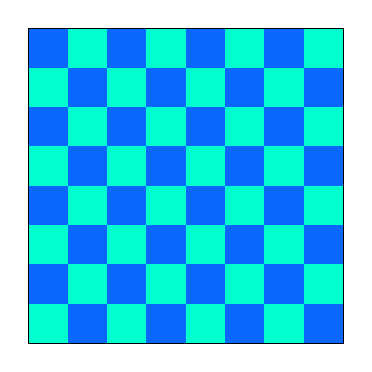
\begin{tikzpicture}[x=1cm,scale=0.5]
    \foreach \x in {0,...,7} \foreach \y in {0,...,7}
    {
        \pgfmathparse{mod(\x+\y,2) ? "lowDensity" : "highDensity"}
        \edef\colour{\pgfmathresult}
        \path[fill=\colour] (\x,\y) rectangle ++ (1,1);
    }
    \draw (0,0)--(0,8)--(8,8)--(8,0)--cycle;
\end{tikzpicture}
    \caption[Chess board pattern]{Chess board pattern with blue squares having a density of 1 person per square meter and turquoise squares having a density of 3 person per square meter.}
    \label{fig:chessBoard-low1-high3-band5}
\end{figure}

The next section will give concrete data that shows how different bandwidths affect the density estimation.

\subsubsection{Effect of Bandwidth}

Using the chess board pattern introduced in the previous section, we will now get a better intuition of the choice of bandwidth. 

\begin{figure}[htbp]
\centering

\begin{subfigure}[c]{.32\linewidth}
    \centering
    \includegraphics[width=\textwidth]{chessBoard-low1-high3-band1-density-subsquares.png}
    \caption{Bandwidth 1 metre}
    \label{fig:chessBoard-low1-high3-band1-cropped}
\end{subfigure}
%
\begin{subfigure}[c]{.32\linewidth}
    \centering
    \includegraphics[width=\textwidth]{chessBoard-low1-high3-band5-density-subsquares.png}
    \caption{Bandwidth 5 metre}
    \label{fig:chessBoard-low1-high3-band5-cropped}
\end{subfigure}
%
\begin{subfigure}[c]{.32\linewidth}
    \centering
    \includegraphics[width=\textwidth]{chessBoard-low1-high3-band10-density-subsquares.png}
    \caption{Bandwidth 10 metre}
    \label{fig:chessBoard-low1-high3-band10-cropped}
\end{subfigure}
%
\caption[Analysed chess board pattern with different bandwidths]{Cropped chess board pattern with blue squares having a density of 1 and turquoise squares having a density of 3. The bandwidth varies on the different subfigures.}
\label{fig:chessBoard-different-bandwidths}
\end{figure}

Let's look at how three different bandwidths change the kernel density estimation of the same data set. \Cref{fig:chessBoard-different-bandwidths} depicts three chess board patterns with varying bandwidths. \Cref{fig:chessBoard-low1-high3-band1-cropped} is very close to the structure of the chess board pattern, but there is some unwanted noise in the blue squares. We would say that the estimation is a little undersmoothed. \Cref{fig:chessBoard-low1-high3-band5-cropped} has a more blurry transition between each adjacent square, which means that the estimation is not really finding the hard transition of the underlying true data. There is however no noise inside each square. We would say that the estimation is a little oversmoothed. In \cref{fig:chessBoard-low1-high3-band10-cropped} we see a clear example of an oversmoothing bandwidth. Each square transition is still somewhat visible, but it is nowhere near the underlying true data.

Every bandwidth in \cref{fig:chessBoard-different-bandwidths} had some problems; Either the bandwidth was too low or too high. We will now try to determine a better bandwidth using the aforementioned SSE method. We iterate through a bandwidth interval from 1 metre to 5 metres with a step of 0.1 metre, because we know that the optimal bandwidth is around that interval. The result of the calculation is that the best bandwidth is 1.4 metre with an SSE of $5745.06$. \Cref{fig:chessBoard-low1-high3-band1.4-cropped} shows a crop of the chess board data with a bandwidth of 1.4 metre. We can see that this bandwidth indeed seems to be optimal; There is no noise inside the blue squares, and the square transitions are still following the underlying structure of the true density data.

\begin{figure}[htbp]
\centering
\includegraphics[width=0.32\textwidth]{chessBoard-low1-high3-band1-4-density-subsquares.png}
\caption[Analysed chess board pattern with bandwidth 1.4]{Cropped chess board pattern with blue squares having a density of 1 and turquoise squares having a density of 3. The bandwidth of 1.4 metres is calculated using a SSE method.}
\label{fig:chessBoard-low1-high3-band1.4-cropped}
\end{figure}

\subsubsection{Bandwidth Summary}

The above sample data is useful for giving an intuition of the effect of different bandwidths, but in order for the bandwidth selection to be useful in practice, one would have to do the bandwidth selection on data that represents the crowd to be analysed.
\subsection{Summary}

We saw in this section, how kernel density estimation can be used to estimate the crowd factors, we wish to visualise for the users of the system. While we must remember that this is only estimation, we consider it to be a precise one. The mathematical definitions of the crowd factors was introduced and integrated with the kernel density estimation.

We also found that choosing the bandwidth is a very important step in the process. While we were unable to settle on a bandwidth, we showed how it can be deducted from a data set. This technique can be implemented, such that once a representative data set is available, we can adjust the bandwidth accordingly.

But a problem still remains. While these formulae might give us the answer we are looking for, we need to consider how they can be implemented in a web application where users expect to have the analysis done in real-time.

%crowd factors


%bandwidth


%analyser link

%% design and planning
\section{Analyser Design}\label{s3:analyser_design}

The analysis of the crowd factors of large events require a great amount of calculations. From the interviews with SmukFest we can expect numbers upwards of 50,000 people during peek hours, and there are many events dealing with much larger numbers of people, such as the Hajj \cite{website:Wikipedia-Hajj2}. If the application is to work on large scales, we need to consider the design of the analyser module, in order to keep the amount of calculations, network communication, and memory use to a minimum.

\subsection{Asynchronous Analysis}
\label{sub:Asynchronous_Analysis}

The first way we reduce the amount of calculations, is to do the analysis asynchronously from user requests. If we were to do a new analysis every time a user wants to see the crowd conditions for a given time period, multiple users requesting real-time analysis would quickly cripple the system. Instead we have a request-handler module, that handles the incoming requests and prepares them for the analyser. In order to fully benefit from this we also have to store completed analyses, such that identical requests can utilise the same results. This prompts the need for a storage module, which stores and catalogues completed analyses. This way the request-handler can bypass the analyser if the requested data is already available in storage, saving computation time.

This architecture allows us, and also require us, to have policies for the request-handler and storage modules. The policy for the request-handler should consider the priority of the incoming requests, whether it be first come first serve, or a priority based system where certain users are prioritised. Another possibility assuming that recently requested heatmaps are saved for some time is to rank requests based on the expected popularity, for instance the newer heatmap the more likely it is to be requested. The storage module also require a policy as to which data to keep and for how long to keep it. Once again different policies can be considered depending on the scope of the system. If we have enough space we can choose to keep all the analysed data, especially if we knew that the system would only run over a certain time period, for instance, the festival. If the system should be able to run indefinitely we would likely prefer to prioritise the data, and only keep a certain amount.

Given the asynchronous design, any data required by the analysis should be retrieved and prepared in advance, so that the analysis does not get unnecessarily delayed. This includes two parts, the first being the retrieval of position data from the aSTEP core, and the other being selection of the points which the analyser will analyse.

\subsection{Supplying Position Data}

Due to the nature of the velocity and heading-direction analysis, data preparation involves a short history of positions to be available. The direct approach of preparing data for each analysis and then deleting it once the analysis has been completed would likely cause an unnecessary amount of request to the aSTEP API. Take the example illustrated in \cref{memposexample} where an analysis is done for the time of $t_0$, where the last couple of positions for $t_{-1}$, $t_{-2}$, and $t_{-3}$ are also prepared. Then afterwards another analysis is done for time $t_{1}$, and we prepare data from $t_0$, $t_{-1}$, and $t_{-2}$. Here it would have been beneficial to retain $t_{-2}$, $t_{-1}$ and $t_{-0}$, since a lot of it overlaps with the analysis of $t_1$. Depending on the policy chosen for the request-handler, the data preparation should accommodate for future requests. Under the assumption that the most recent analysis would be the most requested or that we store all completed analyses indefinitely, it would be preferable to keep position data for the latest $n$ steps, where $t_{-n}$ is the oldest position used for finding the heading-direction and velocity. Different policies for the request handler will however affect the optimal choice of data kept in preparation.

\begin{figure}[htbp]
    \centering
    \begin{tabular}{rcccc}
        \nth{1} analysis: & $t_{-3}$ & $t_{-2}$ & $t_{-1}$ & $t_{0}$ \\
        \nth{2} analysis: & $t_{-2}$ & $t_{-1}$ & $t_{0}$  & $t_{1}$
    \end{tabular}
    \caption{Overlapping data required for analysis.}\label{memposexample}
\end{figure}


\subsection{Selection of Points to Analyse}
\label{s3:select_points}
Now that we have prepared the position data for the analyser, we have to select some points to analyse the local crowd factors for.

We divide the area to analyse into a grid of hexagons. In \cref{sub:kernelDensityEstimation} we assume that people are affected by the crowd factors in a radius away from them, resulting in a circular area of affection. The same assumption can also be used in the representation, meaning that the optimal representation would also display circles. The prblem meanwhile is that it is not possible to make a perfect circular tessellation on a square plane. Meanwhile hexagons have the nice property that a regular tiling can be made with them, i.e. they can be placed in a pattern where they cover an entire area without overlapping nor leaving gaps. While squares also hold this property, we prefer hexagons since they are the closest resembling regular tiling of  a circle with radius of the bandwidth. \Cref{fig:analysis_hexagon_divide} provides an illustration of this. The centre of each hexagon is a point that the analyser should analyse.

\begin{figure}[htbp]
\centering
\begin{tikzpicture} [
    hexa/.style= {shape=regular polygon,
                  regular polygon sides=6,
                  minimum size=1cm, draw,
                  inner sep=0,anchor=south,
                  fill=lightgray}
    ]

\foreach \j in {0,...,4}{% 
     \ifodd\j 
         \foreach \i in {0,...,3}{\node[hexa] (h\j;\i) at ({\j/2+\j/4},{(\i+1/2)*sin(60)}) {.};}        
    \else
         \foreach \i in {0,...,3}{\node[hexa] (h\j;\i) at ({\j/2+\j/4},{\i*sin(60)}) {.};}
    \fi}
\end{tikzpicture}
\caption{Illustration of dividing the area to analyse into a grid of hexagons.}\label{fig:analysis_hexagon_divide}
\end{figure}


\subsection{Lightweight Results}

While we are primarily concerned with reduction of complexity and computation time of the analysis, there are other aspects of the design that require some attention. The amount of data required for a single analysis can reach rather large sizes, and in order to keep network traffic with potentially multiple users to a minimum, the analyser should, as a bi-product of its analysis, reduce the size of a completed analysis. In other words, a lightweight data structure for the results should be conceived. 

The conceived data structure stores the result of the crowd condition analysis along with the matching position, by taking advantage of the uniform distribution of analysed points in a grid. This allows the data structure to only keep track of the global position of one single point and then the distance between points, as well as the dimensions of the analysed area. From this information a client can recreate the grid and start plotting the sequential data accordingly.

This removes the need to send a global position for each point, however it does require the structure to hold every single point in the grid, even if the point is not affected by any person and all its values are zero.

\subsection{Summary}
The asynchronous design of the analyser allows us to divide the analysis into separate parts, which in turn allow for assembly line approach where as much preparation as possible can be done ahead of time. The analyser can run continuously, without being slowed down by communication with data sources. The different parts needs to be implemented with policies which govern their behaviour. The design suggests an implementation where policies can be substituted, in order to easily tailor the system to different uses.

The design also allows for different data structures to be used for communication with the client. Even though we decided for a specific one, by splitting up the analyser from this process the data structure chosen can easily be switched for another in chase the nature of the data changed.

%% implementation
\section{Implementation}
This section will cover how the analyzer was implemented and it's time complexity. Afterwards it will be explained how the visualization of the crowd factors where implemented.

In this section we will cover the important parts of the implementation that was done during this sprint. First we will discuss the implementation of the analyser, and the efforts made towards a faster analysis. We will also briefly cover the implementation of the client side visualisation.

\subsection{Implementation of the Analyser}\label{s3:analyser_implementation}

In order to fully understand the need for a good implementation of the analyser, we start with a quick rundown of the complexity of the unoptimized direct analysis algorithm, which follows the mathematical formulas.

\begin{algorithmic}[1]

\Function{Analyser}{List of Points, List of People, Bandwidth}
\ForAll{points, x}
    \State KernelSum $\gets 0$
    \ForAll{People, P}
        \State KernelSum $\gets$ KernelSum $+$ \Call{Kernel}{P}
    \EndFor
    \State LocalDensity $\gets$ KernelSum $/$ (\Call{Count}{P} $\cdot$ Bandwidth)
\EndFor

\ForAll{points, x}
    \State KernelSum $\gets 0$
    \State VelocitySum $\gets 0$
    \ForAll{People, P}
        \State VelocitySum $\gets$ VelocitySum $+$ \Call{VelocityOf}{P} $\cdot$ \Call{Kernel}{P}
        \State KernelSum $\gets$ KernelSum $+$ \Call{Kernel}{P}
    \EndFor
    \State x.LocalVelocity $\gets$ VelocitySum $/$ KernelSum
\EndFor

\ForAll{points, x}
    \State KernelSum $\gets 0$
    \State TurbuSum $\gets 0$
    \ForAll{People, P}%
        \State TurbuSum $\gets$ TurbuSum $+$ \Call{DirectionOf}{P} $\cdot$ \Call{Kernel}{P}
        \State KernelSum $\gets$ KernelSum $+$ \Call{Kernel}{P}
    \EndFor
    \State LocalTurbulence $\gets$ TurbuSum $/$ KernelSum
\EndFor

\ForAll{points, x}
    \State KernelSum $\gets 0$
    \State PressSum $\gets 0$
    \ForAll{People, P}
        \State VelocityDif $\gets$ (\Call{VelocityOf}{P} $-$ x.LocalVelocity)
        \State PressSum $\gets$ PressSum $+$ \Call{Abs}{VelocityDif}$^2$ $\cdot$ \Call{Kernel}{P}
        \State KernelSum $\gets$ KernelSum $+$ \Call{Kernel}{P}
    \EndFor
    \State LocalPressure $\gets$ x.LocalDensity $\cdot$ (PressSum $/$ KernelSum)
\EndFor
\EndFunction
\end{algorithmic}

%Create points to cover the area.
%
%For each point x:
%    KernelSum <- 0
%    For each person p:
%        KernelSum += KernelFunction(p)
%    x.LocalDensity <- KernelSum / (people * bandwidth)
%    
%For each point x:
%    VelocitySum <- 0
%    KernelSum <- 0
%    For each person p:
%        VelocitySum += VelocityOf(p) * KernelFunction(p)
%        KernelSum += KernelFunction(p)
%    x.LocalVelocity <- VelocitySum / KernelSum
%   
%For each point x:
%    DirectionSum <- 0
%    KernelSum <- 0
%   For each person p:
%       DirectionSum += HeadingDirectionOf(p) * KernelFunction(p)
%        KernelSum += KernelFunction(p)
%    x.LocalTurbulence <- absoluteOf( DirectionSum / KernelSum )
%
%For each point x:
%    pressureSum <- 0
%    KernelSum <- 0
%    For each person p:
%        pressureSum += 
%        kernelSum += kernelFunction(p)
%    x.LocalPressure <- x.LocalDensity * (pressureSum / KernelSum)
%    
%Return Points

This algorithm has a running time of $$O(4\cdot((\text{points} \cdot \text{people}) \cdot 2 \cdot O(KernelFunction)))$$ which might seem as a decent complexity, but considering the constants and the amount of points and people, we need to reduce this.


\subsubsection{Reducing Complexity}

The first thing we need to reduce is the complexity. Removing constant from the notation the complexity itself comes out to $$O(\text{points} \cdot \text{people})$$ which prompts us to reduce either the amount of points or the amount of people.

points can obviously be reduced, but not without also reducing the granularity of the result. But even if we reduce the number of points, we are not able to reduce the complexity. So if we want to reduce the complexity we need to reduce the amount of people iterated through. Considering that the kernel function will return zero for any person further away from the point than the bandwidth, we can reduce the complexity given that a reasonable bandwidth is used. This also relies on the reasonable assumption that people take up space, and that therefore we can only have a certain amount people inside a given bandwidth.
\kanote{færdiggør analysen når vi har en bandwidth}

But before we can utilize this, we need a way to check if a person is further away than the bandwidth, without having to iterate through all the people. Luckily such a way exists in the form of R-trees. An R-tree is a data structure that allows us to do range searches in $O(log_m(n))$ \cite{} \kanote{R-tree kilde + overvej at uddybe lidt}.


\subsubsection{Reducing Constants}

Having reduced the complexity, we still need to reduce the amount of constants in our algorithms run time. We wish to reduce the amount of iterations on the points, as well repeated calculations such as the Kernel values.

%Complexitet
%%

%Minimering af konstanter
%% R-trees
%% Hvorfor det er nice

% Hvorfor regner vi ikke tingene ud hver for sig?
\subsection{Crowd Conditions Visualisation Rendering}\label{sec:own_leaflet_plugin}
\kanote{udvid dette afsnit}

Up till this point we have used different Leaflet plug-in libraries for visualisation, but these libraries are not adequately flexible for the data we have to visualise. We therefore create our own Leaflet plug-in, giving us more flexibility in tailoring visualisations to our needs.

Every Leaflet plug-in library we tried has its own assumption on how the data should be visualised, and this assumption does not satisfy our needs. For example, all libraries used a global scaling of densities, meaning the density of a point depends on the density of other points. Additionally, we had no control over the shapes used in the visualisations.

Because of this, we decided to create our own Leaflet plug-in based on Leaflet.heat. The goals of this plug-in is to allow us to experiment with different visualisation techniques. By creating our own plug-in, we have complete control of how the data is drawn on the map. This means that we can render the visualisations in a very specific fashion that suits our needs.


%% conclusion
\section{Conclusion of Sprint}
The third sprint started on March \nth{2} and ended on the April \nth{21}. The work presented in this sprint is primarily the development of the central component of the project, namely the analyser. Based upon the requirement that the system needs to be able to analyse the crowd conditions, we incorporated and adjusted methods of utilising position data to estimate crowd conditions. This entailed a deeper understanding of the nature of the crowd factors, and how the mathematical modelling represents it, which was required in order to tailor it to our requirements.

While our sources of inspiration have primarily done analysis on past events, our requirement for near real-time analysis prompted us to design our application around the analyser, in order to increase our computational output. This incentive was passed through to the implementation, which also had the primary concern of optimising the analysis for speed. The results of both the design and implementation are considered successful, as they both manage to considerably reduce the required time for analysis.

There was also a focus on altering the calculations for the crowd factors to fit the results found in other sources, in order to compare values found in the analyser with empirically found levels of hazard found in other research. This was also successful, as all factors calculated in the analyser is on relative form.

While the calculations are considered correct in the mathematical sense, we have yet to evaluate the analysis in a practical setting.